\documentclass{article}

\usepackage{graphicx}

\title{GenetiCHR tutorial}
\author{Christian Theil Have\\ cth@ruc.dk}

\begin{document}

\maketitle

\section{Introduction}

GenetiCHR is a library for genetic computing written in CHR/Prolog. It is designed primarily to be simple to understand and easy to use, performance being a secondary concern. 

Implementing a genetic algorithm in GenetiCHR is a simple matter of implementing a few callback functions that must implement crossover, mutation, fitness calculation
and generation of the initial generation. The library contains a few common crossover and mutation functions for lists/strings and trees.

The library gives the user a number of choices with regard to parameters of the genetic algorithm such as generation size, fitness threshold and selection method (tournament or elitism).


The framework is available for download at,
\begin{verbatim}
http://github.com/cth/GenetiCHR
\end{verbatim}

\section{Overview of the framework}

The core of the framework is in the file \verb|genetichr.pl|. In the constraint a generation of individuals are maintained as \verb|individual/4| constraints. These constraints are iteratively refined
in each iteration of the algorithm. An iteration has three phases. The current phase is indicated by the \verb|phase/1| constraint.

\begin{enumerate}
\item Mutation phase: A percentage of individuals in current generation is randomly selected for mutation. The mutation callback rule is called and the mutated individuals are inserted into the current generation.
\item Crossover phase:  A percentage of pairs of individuals are selected for crossover. The crossover callback rule is called and two offspring individuals are inserted into the current generation. Note that also mutated individuals may be selected for crossover.
\item Selection phase: After mutation and crossover the number of individuals in the current generation $m$, exceeds the allowed population size, $k$. In the selection phase $k$ individuals are selected for survival and $m-k$ individuals are eliminated. The choice of which individuals should survive depends on the scheme indicated \verb|selection_mode/1| - which may be either \verb|elitism| or \verb|tournament|. Both schemes uses the fitness callback rule to rank individuals.
\end{enumerate}

After selection, there might be an individual with a fitness above the threshold or the generation threshold might have been reached. In both cases, the algorithm terminates and prints the individuals of the current generation. If neither is the case, the process loops, starting the next iteration with a new mutation phase.

\subsection{Initialization of the framework}
\label{sec:initialization}

Before starting the evolutionary process certain parameters must be set by the user. This is done by adding certain constraints to the store:
\begin{itemize}
\item \verb|population_size/1| - an integer which determines how many individuals survive each generation. 
\item \verb|mutation_rate/1| - a floating point number $[0..1]$ which is the probability with which individuals are selected for mutation.
\item \verb|crossover_rate/1| - a floating point number $[0..1]$ which is the probability with which a particular pair of individuals are selected as parents in a crossover.
\item \verb|fitness_threshold/1| - an number float/integer. When the fitness of any individual reaches/exceeds this number, the algorithm terminates.
\item \verb|generation_threshold/1| - an integer number determines the maximal number of iterations that the algorithm will run for. 
\item \verb|selection_mode/1| - see section \ref{sec:selection_modes}.
\end{itemize}

\subsubsection{Selection modes}
\label{sec:selection_modes}

A selection mode is set by adding a \verb|selection_mode| constraint to the store. The two choices are \verb|selection_mode(elitism)| and \verb|selection_mode(tournament)|. 

With elitism, the $k$ best individuals of the generation (after mutation and crossover) are deterministically selected for survival, where $k$ is the population size indicated with the \verb|population_size/1| constraint. 

In tournament selection $k$ "tournaments" are created where the individuals are pitted against each other. Each individual is assigned to a random tournament. For each tournament, the individual with the highest fitness is selected for survival. Note that this kind of selection has a stochastic element and might therefore eliminate very fit individuals which would have survived in elitism. This can be an advantage as it may allow the algorithm to escape from local minima and explore the search space better. 

The optimal choice of selection scheme depends on the nature of the problem.

\subsection{Definition of callback rules}

Whenever a new individual needs to be created, the fitness of an individual needs to be calculated, an individual needs to be mutated or a pair should be crossed over, callback rules defined by the user are used to accomplish the goal.
To implement an genetic algorithm using the framework, four callback rules needs to be implemented.

\begin{itemize}
\item \verb|cb_create_individual(-Genome)| : Called to create individuals in the initial generation. This will be called as many times as there are individuals in the population (indicated by \verb|population_size/1|, see section \ref{sec:initialization}). It is the job of the user to implement the rule such that \verb|Genome| is unified to a representation of an individual.
\item \verb|cb_calculate_fitness(+Genome,-Fitness)| : Called in the selection phase to calculate the fitness of an individual. \verb|Fitness| must unify to a number (either float or integer). Higher numbers indicate better fitness. 
\item \verb|cb_mutate(+Genome, -MutatedGenome)| : Called in the mutation phase when individuals are selected for mutation. \verb|MutatedGenome| must be unified to a mutated genome, but the mutation method is entirely up to the user. For a choice of common mutation rules, see section \ref{sec:mutation_rules}
\item \verb|cb_crossover(+Parent1,+Parent2,-Child1,-Child2)| : Called to crossover two individuals. The process yields two children. The crossover method up to the user. Some commonly used crossover rules are available as a convenience, see section \ref{sec:crossover_rules}.
\end{itemize}

\subsection{Mutation rules}
\label{sec:mutation_rules}

The library contains some rules which implements some basic approaches to mutations. These mutation rules assumes that the genome is represented as Prolog list. These rules are implemented in the file 
\verb|mutation.pl|.

\bigskip
\noindent
\verb|single_point_mutate(-Genome,+MutatedGenome,-Alphabet)|\\
One random element of the \verb|Genome| list is mutated to one of the elements of the \verb|Alphabet| list, selected at random.\\

\bigskip
\noindent
\verb|multi_point_mutate(-Genome,+MutatedGenome,|\\
\verb|                   -Alphabet,-PointMutationProb)| \\
Any element of the  \verb|Genome| list is mutated with a probability of \texttt{PointMutationProb}. 
The mutation outcomes are randomly selected from the \verb|Alphabet| list with uniform probability.

\subsection{Crossover rules}
\label{sec:crossover_rules}


Some common crossover approached have been implemented as part of the framework. To use them, just call them from the user-defined \verb|cb_crossover_callback| function.\footnote{Some of the contents of this section has been derived from wikipedia entry on crossover functions.}

\subsubsection{One-point crossover}

\verb|one_point_crossover(-MotherGenome,-FatherGenome,+Child1Genome,+Child2Genome)|
\medskip

One point cross over assumes equal length of genomes. A single crossover point on both parents' organism strings is selected. All data beyond that point in either organism string is swapped between the two parent organisms. The resulting organisms are the children, see figure \ref{fig:one_point_crossover}.
\begin{figure}[htb]
\caption{One-point crossover}
\label{fig:one_point_crossover}
\centerline{\scalebox{0.8}{ 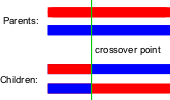
\includegraphics{SinglePointCrossover.png} } }
\end{figure}

\subsubsection{Two-point crossover}

\verb|two_point_crossover(-MotherGenome,-FatherGenome,+Child1Genome,+Child2Genome)|
\medskip

Two-point crossover calls for two points to be selected on the parent organism strings.  Everything between the two points is swapped between the parent organisms, rendering two child organisms.
See illustration in figure \ref{fig:two_point_crossover}

\begin{figure}[htb]
\caption{Two-point crossover}
\label{fig:two_point_crossover}
\centerline{\scalebox{0.8}{ 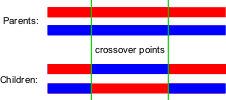
\includegraphics{TwoPointCrossover.png} } }
\end{figure}

\subsubsection{Cut-and-splice crossover}
\label{sec:cut_and_splice}

\verb|cut_and_splice(-MotherGenome,-FatherGenome,+Child1Genome,+Child2Genome)|
\medskip

The "cut and splice" approach, results in a change in length of the children strings. The reason for this difference is that each parent string has a separate choice of crossover point.
Illustration is shown in figure \ref{fig:cut_and_splice}.

\begin{figure}[htb]
\caption{Cut-and-splice crossover}
\label{fig:cut_and_splice}
\centerline{\scalebox{0.8}{ 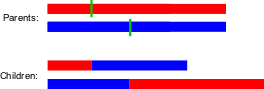
\includegraphics{CutSpliceCrossover.png} } }
\end{figure}

\subsubsection{Uniform crossover}

\verb|uniform_crossover(-MotherGenome,-FatherGenome,|\\
\verb|                  +Child1Genome,+Child2Genome,-SwapProbability)|
\medskip

In the uniform crossover scheme individual elements in the genome lists are compared between two parents. The elements are swapped with a fixed probability (\verb|SwapProbability|). A typical choice
for \verb|SwapProbability| is \verb|0.5|.

\subsubsection{Binary tree crossover}

\verb|binary_tree_crossover(-Parent1,-Parent2,+Child1,+Child2)|

This method works on (binary) trees rather lists and is particularly useful for genetic programming in a lisp like setting. A random node (subtree) is selected in each of the parent trees. In the child trees the 
these subtrees are then swapped. See figure \ref{fig:binary_tree_crossover} for an illustration.

\begin{figure}[htb]
\caption{Binary tree crossover}
\label{fig:binary_tree_crossover}
\begin{verbatim}
 Parent1: [mul,2,[plus,a,b]]
 Parent2: [plus,[mul,a,b],a]
 Child1: [mul, 2, b],
 Child2: [plus, [mul, a, [plus, a, b]], a]
\end{verbatim}
\end{figure}

\section{A simple example: Evolution of a string}

This example is trivial and not a very interesting application of genetic algorithms. However, it illustrates the basic principles of developing
a genetic algorithm using GenetiCHR. The example may be found in the GenetiCHR library in \verb|examples/evolve_string/|.

The idea is to evolve a number of individual strings, represented as a list of character codes, into the string we are looking for. We define the 
target string to be, 
\begin{verbatim}
target_string("cafebabe").
\end{verbatim}

Also, we define the alphabet we wish to use for these strings. This delimits the search-space,
\begin{verbatim}
characters("abcdef").
\end{verbatim}

\subsubsection{Definition of callback rules}

Four callback rules for creation of individuals, mutation, crossover and fitness calculation,  needs to be defined. We go through each in turn.

\paragraph{Creation of individuals,}

\begin{verbatim}
cb_create_individual(Genome) :- create_random_string(Genome).
\end{verbatim}
This rule is called every time a new individual should be created for inclusion in the initial generation. \verb|population_size/1| determines how many times it will be invoked.
It just calls \verb|create_random_string/1| which creates a random list of character codes from the defined alphabet,
\begin{verbatim}
create_random_string([]) :-  random(Prob),  Prob < 0.1, !.  % Stop
create_random_string([Char|Rest]) :-
  create_random_character(Char),
  create_random_string(Rest).

create_random_character(Char) :-
  characters(Chars),
  random(P),
  length(Chars,NumChars),
  CharIndex is round(P * (NumChars-1)),
  nth0(CharIndex,Chars,Char).
\end{verbatim}

\paragraph{Mutation} uses the library \verb|multi_point_mutate| rule (see section \ref{sec:mutation_rules}), 
\begin{verbatim}
cb_mutate(Genome, MutatedGenome) :-
  characters(C),
  multi_point_mutate(Genome,MutatedGenome,C,0.1).
\end{verbatim}

After a call to \verb|cb_mutate|, \verb|MutatedGenome| will have mutations in 10 percent of all its bases on average. Note that bases are only 
mutated to characters from the defined alphabet.

\paragraph{Crossover} uses the library \verb|cut_and_splice| rules, see section \ref{sec:cut_and_splice}.

\begin{verbatim}
cb_crossover(GenomeFather,GenomeMother,ChildGenome1,Child2Genome) :-
  cut_and_splice(GenomeFather,GenomeMother,ChildGenome1,Child2Genome).
\end{verbatim}

Note that we cannot easily use one-point crossover, which assumes that the parent genomes are of equal length, since in our initial generation individuals are generated
with random lengths.

\paragraph{Fitness calculation} is calculated as the negative Levenshtein/edit distance\footnote{The Levenshtein distance is defined as the minimal number of character substitutions, insertions and deletions needed to transform one string into an other.} to the target string,

\begin{verbatim}
cb_calculate_fitness(Genome,Fitness) :-
  target_string(Target),
  atom_codes(Atom1,Target),
  atom_codes(Atom2,Genome),
  levenshtein(Atom1,Atom2,Distance),
  Fitness is 0 - Distance.
\end{verbatim}

\paragraph{Initialization}

To initialize the algorithm we create a rule which adds all the necessary constraints as indicated in section \ref{sec:initialization}:

\begin{verbatim}
run_example :-
  population_size(50), 
  mutation_rate(0.1),
  crossover_rate(0.2),
  fitness_threshold(0),
  generation_threshold(1000),
  selection_mode(elitism), 
  phase(initialization). 
\end{verbatim}

Note, that the last constraint \verb|phase(initialization)| effectively starts the algorithm with a first generation.

We can now start the process by loading the file and calling the goal \verb|run_example|. 

\subsection{Running the example}

The example runs in SWI prolog. It may be a good idea to load SWI with a large global and local stack, e.g. 
\begin{verbatim}
swipl -G128M -L128M
\end{verbatim}

\noindent
Once we have started SWI prolog, we can load the example, 
\begin{verbatim}
?- [evolve_string].
\end{verbatim}

\noindent
We can now run the example by calling the goal \verb|run_example|:

\begin{verbatim}
?- run_example.
cb_create_individual: debdbcfbfcece
cb_create_individual: deeeedbdc
....
cb_create_individual: ba
cb_create_individual: eec
Generation 0
  - mutation phase
  - cross over phase
  - selection phase
Evolution cycle done. Starting on generation 1
Best individual: individual(64, 1, [97, 101, 98, 98], -4)
Average fitness of generation: -6.26
  - mutation phase
  - cross over phase
  - selection phase
Evolution cycle done. Starting on generation 2
Best individual: individual(204, 2, [99, 99, 100, 101, 98, 98, 101], -3)
Average fitness of generation: -5.62
  - mutation phase
  - cross over phase
  - selection phase
...
...
Evolution cycle done. Starting on generation 27
Best individual: individual(2538, 26, [99, 97, 102, 97, 101, 98, 97, 98, 101], -1)
Average fitness of generation: -2.24
  - mutation phase
  - cross over phase
  - selection phase
Individual with fitness threshold 0 found. Terminating.
Best individual: individual(2720, 28, [99, 97, 102, 101, 98, 97, 98, 101], 0)
Average fitness of generation: -2.14
\end{verbatim}

The average fitness of each generation is reported and the best individual in the generation is displayed in each iteration. Note that an \verb|individual| constraint
has four elements: The first is the unique id of the individual, the second is the generation in which the individual was created, the third is the genome of the individual
and the fourth is its fitness.

Finally, in generation 28, a suitable individual is found, causing the process to terminate. You can verify that the sequence of character codes correspond to the string we were looking for using, 

\begin{verbatim}
?- atom_codes(String,[99, 97, 102, 101, 98, 97, 98, 101]).
String = cafebabe.
\end{verbatim}

\end{document}